\documentclass{article}
\usepackage{graphicx}
\usepackage[nottoc,numbib]{tocbibind}
\usepackage[a4paper, total={6in, 8in}]{geometry}
\usepackage{subcaption}
\usepackage{titling}
\usepackage{float}
\usepackage{wrapfig}
\newcommand{\subtitle}[1]{%
  \posttitle{%
    \par\end{center}
    \begin{center}\large#1\end{center}
    \vskip0.5em}%
}
\newcommand{\myparagraph}[1]{\paragraph{#1}\mbox{}\\}

\title{Topics in Privacy \& Security}
\subtitle{Ransomware}
\author{Y1481702}
\date{\today}
\setlength\parindent{0pt}
 
\begin{document}
\begin{titlepage}
\clearpage\maketitle
\thispagestyle{empty}
\tableofcontents
\end{titlepage}

%In answering each part of the question, consider the level of IT expertise of the personnel that your answer is aimed at, and the security mechanisms they are able to implement.
%Your answer to this question must not exceed six A4 pages (minimum font size 11pt) plus references.

%APPROX ONE PAGE PER 10 MARKS:

\section{Technical Report}% 30 Marks - 3 pages
\subsection{Introduction}
%Write a technical report the organisation's IT managers about the structure of ransomware attacts, about the dangers these attacks post to healthcare providers, and about the prevention, detection and response mechanisms they should implement on the organisation's computers to best protect them against such attacks.

%BACKGROUND- Newsy stuff
2017 saw a significant rise in frequency of ransomware attacks[CITE], with WannaCry\cite{wannacry_reuters, wannacry_bbc} and NotPetya\cite{petya_independent} being two particularly damaging examples.
These attacks becoming more prevalent is likely driven by the rise of cryptocurrencies, such as Bitcoin, which are more difficult to trace than traditional bank transfers.
Furthermore, as more essential appliances, such as thermostats and smoke detectors, become dependent on complex software and, with the internet of things providing new possibilities for remote attack, it is likely this trend will continue.
\\\\%WHAT HAPPENS?
At a high-level the attack works as a form of protection racket, with profit as the key motivation\cite{mcafee_2018}.
%-McAfee Labs 2018:\cite{mcafee_2018}
%"cyber sabotage and disruption of organisations"
%profit is the key driver of ransomware: criminals aim to make money from inconveniencing a user
%unscrupulous competitors or criminals (protection racket)
The attack aims to violate the security goal of availability.
Users are denied access to vital systems and services and offered the option to pay to get around this inconvenience. As with other criminal ransom acts, there is absolutely no guarantee that paying the ransom will return the files successfully\cite{ncsc_mitigating_malware}. 
Indeed doing so also incentivises the hacker to produce more attacks in the future.
A recent report has even shown that as little as 19\% of ransomware victims who pay the ransom may actually get their files back\cite{cyberedge_group, forbes_cyberedge}. As such, this kind of attack also violates the goal of integrity as data and software is irreversibly modified.
It should also be noted that while ransomware does not specifically threaten the goal of privacy and confidentiality, it could be used to disguise some form of dual layer attack which does.
\\\\%technical explanation
%What does ransomware actually do:
%encrypts files -> one way transformation, unless key is known
There are a number of ways in which ransomware may attempt to deny access to a system, the most effective of these being to encrypt files on the computer harddrive. 
Encryption uses one-way functions which are computationally hard to reverse, so attempting to restore the data without knowing the key used to encrypt it is \textbf{not} an option.
All files including software, documents and other data may be affected potentially causing a complete loss of the computer.
This technique is what made the WannaCry and NotPetya so efficacious.
%what other methods are there?
Another type of ransomware, known as locker ransomware, may leave files untouched in favour of denying the user access to their desktop and programs. In this case it may be possible to recover critical files from the machine, but a clean restore from a backup may still be preferable.
\\\\%LATEST DEVELOPMENTS
%Ransomware need not ALWAYS be self-multiplying.. but when it is, it can be particularly dangerous!
The latest strains of ransomware have also begun to include the ability to self-multiply meaning they fall under the category of a computer virus. This makes them especially problematic for businesses as they can easily spread across internal networks infecting multiple machines and encrypting a vast number of files.
%stopping this early is difficult but necessary!
%ransomware as a distraction from other attacks- data theft (citation?)
\\\\%RELATE THIS ALL TO HEALTHCARE
%structure of ransomware:
As mentioned above, the latest ransomware are self-multiplying and will therefore not discriminate between businesses and important services such as healthcare.
While ransomware has demonstrated to businesses any of their electronic data may be important\cite{security_breaches_survey} and many have opted to pay the ransom for its recovery, it is hoped that the value of medical data has never been in question.
%talk about surveys:
%-Cyber Security Breaches Survey 2017\cite{security_breaches_survey}
%	ransomware has highlighted the VALUE of any electronic data other than personal/financial data
%		the value of this data for health organisations was likely ALREADY known
%DOES THIS HAVE ANY HEALTHCARE SPECIFIC PROBLEMS?
In the healthcare industry, it is particularly important to defend against any violations of availability.
For obvious reasons, timely access to medical data may be the difference between life and death for some patients.
It is likely be dangerous to run surgeries without full access to patient's medical data or even to blood transfusion or organ donation databases.
%show examples of this?

%NB.:
%An ERROR is a mistake by a human
%A FAULT occurs because of this mistake- i.e. incorrect command/process is run
%A FAILURE is a departure from the required behaviour
\subsection{Prevent}
Once ransomware has access to files on the system, it may be difficult if not impossible to recover the files. Therefore the most effective solution to ransomware is to prevent it taking hold altogether. While it is impossible to ensure that every user of the network is behaving responsibly at all times, sensible steps can still be taken to ensure that the actions of any individual have minimal impact.
\\\\
%Malware:
Ransomware can enter a system in the same way as any other form of malware.
Social engineering is the successful, and thus most common, form of attack vector for home users and organisations alike. %cite?!
Phishing may be used to encourage users to 
%defend against by spam/web filters, educating users

baiting (infected USB drives, etc.)
%defend against by ensuring physical building security

can spread by downloads (as above)
or self-replication via internal or external networks
\\\\
Firstly, keeping operating systems and other software up-to-date ensure that the latest security updates are installed. It's particularly import to ensure that any operating systems are still being supported with new security fixes.
While extended support for Windows XP was dropped back in April 2014, it is estimated that 3.3\% of Windows PCs are still running this OS, which translates to approximately 140 million machines\cite{statcounter}.  The WannaCry vulnerability was patched in Windows 7, 8.1 and 10 security updates\cite{wannacry_patch2, wannacry_patch, windows10march} two months before the ransomware took hold so this action would have prevented much of the attack's impact. While it is necessary to test major updates to ensure important software is not affected and data can be migrated, support expiry dates are announced years in advance\cite{microsoft_lifecycle_factsheet}, so there should be plenty of time to prepare for this. The cost of upgrade should \textbf{never} overule the requirement to ensure system security, especially when patient's data is involved.%cite example for this?
\\\\
Ensuring tight access control should also help to minimize the impact of ransomware. Minimizing users' access to only the assets which they absolutely require will ensure that 

 Ensuring users only have read access, (read access only where necessary) should minimize access of users to corrupt data
review this regularly

\subsection{Detect}
Once a ransomware attack has taken hold, its important to detect and stop it before serious widespread damage can be done.
\\\\
Security controls can be employed to detect ransomware.
In particular, detecting altering of files- ransomware may attempt to modify ANY/ALL files on the system
Detect virus signatures, actions beyond specifications, statistical changes?

Anti-virus software (keeping it up to date regularly)
still may not be particularly effective

Once an attack has been discovered, all affected PCs and network connections from them should be shut down immediately.

\subsection{Recover}
%prevention, detection and response mechanisms:
Once ransomware has taken hold, the system can only be recovered if backups have been made. Backups should be regular and stored offline, away from any network.
While regular backups must be kept as a last resort, prevention and early detection is preferable as recovering a whole system from a backup may take considerable amounts of time.
\\\\
The National Cyber Security Centre recommend the following steps to recover from ransomware\cite{ncsc_mitigating_malware}:
\begin{itemize}
	\item immediately disconnect infected computers from the network, by:
	\begin{itemize}
		\item turning of Wi-Fi
		\item unplugging ethernet cables
	\end{itemize}
	\item format or replace hard drives and reinstall the OS
	\item connect the device to a clean network to download, install and update the OS and all software
	\item install, update and run antivirus software
	\item monitor network traffic and run antivirus scans to identify remaining infection
\end{itemize}

%--look into projects such as NoMoreRansom and Cyber Threat Alliance
\textit{N.B. As much of this report regards recent events, information has been taken from reputable news sources and trusted security organisations where possible.
Where this has not been possible, multiple sources have been provided in order to provide further assurance of the correctness of statements.}

\section{Email}
\subsection{Memo}% 20 Marks - 2 pages 
%Write a memo that the IT managers should email to healthcare personnel who are not IT experts, to warn them about ransomware, to inform them about ways to prevent ransomware attacks, and to advise them what to do if they are affected by such an attack. The memo must only cover the personnel’s use of computers belonging to the organisation and located on the organisation’s premises.

%explanation and appeal for help!
%get attention- users need to be aware of the danger:
%WannaCry brought the NHS to a standstill
In 2017, 48 NHS trusts were brought to a standstill by ransomware. The attack took down the trust's computer systems meaning patient data became complete inaccessible resulting in cancelled appointments and even surgeries\cite{wannacry_bbc}. As well as crippling the NHS, the attack also took down schools, large manufacturers and even banks with an estimated 200,000 computers across 150 countries being affected according to Europol\cite{wannacry_reuters}. Clearly we need to do everything we can to defend against such attacks and \textbf{we need your help}.

\begin{wrapfigure}{l}{0.45\textwidth}
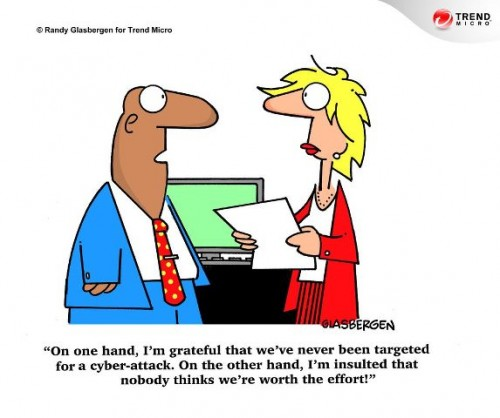
\includegraphics[width=0.45\textwidth]{Figures/Cartoon}
\caption{Cyber Security Cartoon\cite{cartoon}}
\label{Cartoon}
\end{wrapfigure}

\begin{wrapfigure}{l}{0.45\textwidth}
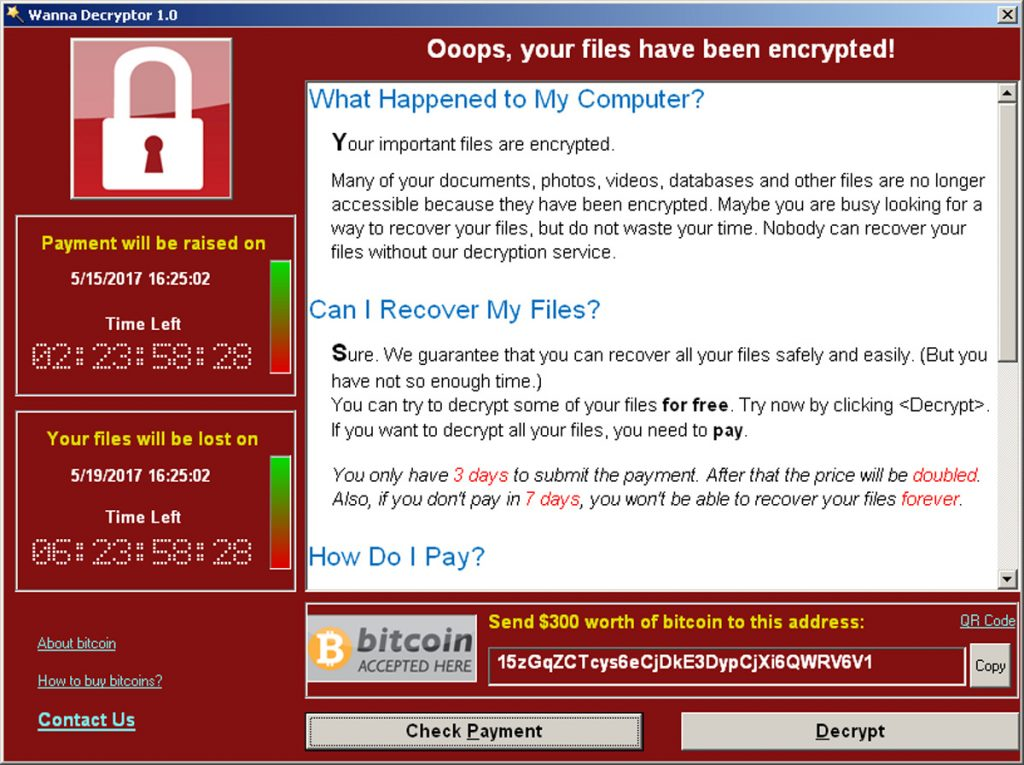
\includegraphics[width=0.45\textwidth]{Figures/wannacry}
\caption{WannaCry Ransomware}
\label{wannacry_decryptor}
\end{wrapfigure}

%background of how computers get infected and what ransomware does
Ransomware attacks that we have seen so far do not distinguish between targets. Their aim is to restrict users from accessing their data or devices and force them to pay a fee to regain entry.
\\\\
%analogy
%how the users can help
%prevent: same as other malware attacks: trojan horse, datatheft
As with other computer viruses that you may be aware of, ransomware often comes disguised as other programs. You will remember from your cyber security training that viruses may come as email attachments or as downloads from unscrupulous websites.

We implore you \textbf{not} to:
\begin{itemize}
	\item interfere with automatic software updates scheduled by system administrators
	\item run or install software that has not been vetted by system administrators
		if you would like additional software to be installed, please contact your service desk
	\item plug \textbf{unknown} devices, such as USB drives, into your computer
\end{itemize}

%IF ATTACKED
%MAIN STEPS
If you are victim of a ransomware attack, you need to act \textbf{quickly} to stop the problem spreading to other users:
\begin{itemize}
	\item \textbf{Don't panic!}
	\item \textbf{Don't} attempt to pay any ransom demands.
	\item Switch off and unplug your PC immediately.
	\item Contact IT support as soon as possible.
\end{itemize}

%CONCLUSION & FOLLOW UP
If you have any follow-up questions regarding ransomware or cybersecurity in general, please do not hesistate to reply to this email. We're more than happy to explain anything further and we'd love to hear your suggestions on how to further engage the community.

\subsection{Justification}% 10 Marks - 1 page
%Write a justification for the information included in the memo from part (ii) of the question, and for how you organised this information. The aim of this justification is to convince the IT managers that the memo they will send is going to be effective.
Care has been taken to aim the email at its target audience: healthcare professionals are often well educated, but may have minimal knowledge or interest in the area of digital security.

As such, the first few lines have been designed to grab the attention of the reader by informing them of the significant impact ransomware has had on similar organisations around the world.
\\\\
Appealing to the user directly - makes clear to the reader which actions they are responsible for\\
Using plurals everywhere else - makes clear this is a problem for the whole organisation and make the user feel comfortable discussing with others if they have questions
\\\\
Graphics such as 
	screenshots of previous ransomware
	%help the user know what to expect if they are attacked
	fun cyber security cartoon
	main steps:
help to break up the text.
\\\\

%which information included
%how it is organised

As users may not be particularly interested in the subject of the email, it has been kept as short as possible, while still including the necessary facts.
If the email becomes too long or uses too many technical words, it is unlikely that employees will read it.
%kept short and to the point, but including necessary facts
	%too long and users are unlikely to read it (cite?)
	%mention Industry experience as justification here?
	%fun diagram or cartoon to draw readers in ?
	%healthcare personnel are often well educated though, so don't OVER simplify

While ransomware is a particularly new threat, the email assumes that the reader is familiar with other types of malware from previous communications and cyber security training.
%most large companies offer some form of cyber security awareness training
This is commonplace, and I have had to under take this myself during industrial placements.

%refer to BS EN ISO standards?
NCSC recommendations
relate this to the technical report in previous section

As analogy has been used to help the users relate to the explanation
%healthcare analogy?
\\\\
At the end of the email, the main actions that the user will need to take in the event of being hit by a ransomware attack have been bulletpointed, and repeated in order to ensure that the user knows these are the key take aways from the memo.
%it is important that the users REMEMBERS these takeaways as speed is of the essense in stopping the spread of ransomware, AND they may not be able to access this email after the attack
%takeaways have been kept to a minimum, users need to know the immediate actions to take- i.e. switch off their PCs and CONTACT IT support..
The user has also been encouraged to ask any questions that might occur to them as a result of the email. This will hopefully result in some feedback that can help us to judge if the email has been understood by the audience.
\\\\
This will be particularly useful in this case as while every effort has been taken to ensure that this memo is suitable for the target audience, it would be a good idea to test it on a member of this audience before sending it out. As this is a university Open Assessment, I have been unable to do this in this instance.

\newpage
\raggedright
\bibliography{Report}{}
\bibliographystyle{ieeetran}
%\newpage
%\section{Appendix}

\end{document}